\documentclass[11pt]{article}

\usepackage{hw_style}

% Set due date for this homework (updated to 2025)
\setduedate{11}{26}

% Setup homework number and header
\hwnumber{8}

\begin{document}

\begin{hwproblem}{}
请类比课堂直角坐标系和柱坐标系的演算, 导出球坐标系(spherical coordinate)下梯度算符$\nabla$的表达式为
\[
\nabla f=\frac{\partial f}{\partial r} \mathbf{e}_r+\frac{1}{r} \frac{\partial f}{\partial \theta}
 \mathbf{e}_\theta+\frac{1}{r \sin \theta} \frac{\partial f}{\partial \varphi} \mathbf{e}_\varphi
\]
\end{hwproblem}

\vspace{0.5cm}

\vspace{2em}

\begin{hwproblem}{}
 对于$f(x) =x^2 y$, 如图所示的三条路径, 请推导验证
$\int_a^b d f=f_{l_b}-f_{l_a}=\int_a^b \nabla f \cdot \mathbf{d l}$
成立, 其中路径1和路径2为折线, 路径3为直线.
\\
\centering
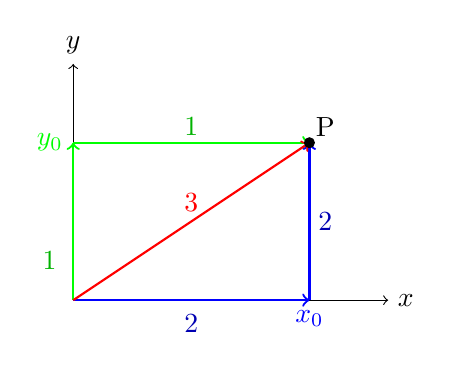
\begin{tikzpicture}

% Draw the axes
\draw[->] (0,0) -- (4,0) node[right] {$x$};  % x-axis
\draw[->] (0,0) -- (0,3) node[above] {$y$};  % y-axis

% Draw the box
% Green path: annotate as path 1 and 2
\draw[->, green, thick] (0,0) -- (0,2) node[left] {$y_0$};
\node[green!70!black] at (-0.3,0.5) {1};
\draw[->, green, thick] (0,2) -- (3,2) node[midway, right] {};
\node[green!70!black] at (1.5,2.2) {1};

% Blue path
\draw[->, blue, thick] (0,0) -- (3,0) node[below] {$x_0$};
\node[blue!70!black] at (1.5,-0.3) {2};
\draw[->, blue, thick] (3,0) -- (3,2) node[midway, right] {};
\node[blue!70!black] at (3.2,1) {2};
% Diagonal line
\draw[->, red, thick] (0,0) -- (3,2) node[midway, above] {3};

% Mark point P
\fill (3,2) circle (2pt);
\node at (3.2,2.2) {P};

% Additional labels for the diagram
% \node at (1,-0.3) {1};
% \node at (0.3, 0.8) {2};
\end{tikzpicture}

\end{hwproblem}

\vspace{0.5cm}
  

\begin{hwproblem}{}
请证明向量等式
\begin{itemize}
  \item [(1)]$$
(\mathbf{A} \times \mathbf{B}) \cdot \mathbf{C}=(\mathbf{B} \times \mathbf{C}) \cdot \mathbf{A}=(\mathbf{C} \times \mathbf{A}) \cdot \mathbf{B},
$$
\item [(2)] 
 $$
\nabla \cdot(\mathbf{A} \times \mathbf{B})=\mathbf{B} \cdot(\nabla \times \mathbf{A})-\mathbf{A} \cdot(\nabla \times \mathbf{B}).
$$
\end{itemize}

\end{hwproblem}

\vspace{0.5cm}

\begin{hwproblem}{}
请证明
\begin{itemize}
  \item [(1)] $$
\int_V \nabla f d V=\oint_S f d \mathbf{S}
$$
  \item [(2)] $$
  \int_{\mathrm{V}} \nabla \times \mathbf{F} d \mathrm{V}=-\oint_S \mathbf{F} \times d\mathbf{S}$$
  \item [(3)] $$\oint_L f d\mathbf{l}=-\int_S \nabla f \times d\mathbf{S}$$
\end{itemize}
提示: 考虑 $\mathbf{A} = \mathbf{i} f$ 和$\mathbf{A} = \mathbf{i} \times \mathbf{F}$,
其中$\mathbf{i}$为单位向量.
\end{hwproblem}

\vspace{0.5cm}
   
% \begin{hwproblem}{}
%   整数$m$阶贝塞尔方程(Bessel's equation)
%   $$
%     x^2 y^{\prime \prime}+x y^{\prime}+\left(x^2-m^2\right) y = 0, 
%   $$
% 的Laplace变换($m = 0$)为一阶常微分方程
%   $$
%    (p^2 + 1) f'(p) + pf(p) = 0.
%   $$
%    试求解$f(p)$.
% \end{hwproblem}

% \vspace{0.5cm}

% \begin{hwproblem}{}
% 求$$
% (2x + e^{y^2}) dx + (2xy e^{y^2} -2y ) dy = 0
% $$
% 的通解.
% \end{hwproblem}

% \vspace{0.5cm}
  



  
  


% % \begin{hwproblem}{7}
% % \end{hwproblem}

% \vspace{0.5cm}

% % \begin{hwproblem}{8}
% % \end{hwproblem}

% \vspace{0.5cm}

% % \begin{hwproblem}{9}
% % \end{hwproblem}

% \vspace{0.5cm}

\hwrequirements

\end{document}